\section{Data handling}

By taking a first look at the data and the statement, we quickly found the missing power values represented by a -1 in the \verb|TARGETVAR| column of all the \verb|Y_i.csv| files. We used this specific -1 value to identify and split our training/test sets. We then wanted to check our files for outliers. We used boxplots to begin investigate the outliers topic :

\begin{figure}[!h]
    \centering
    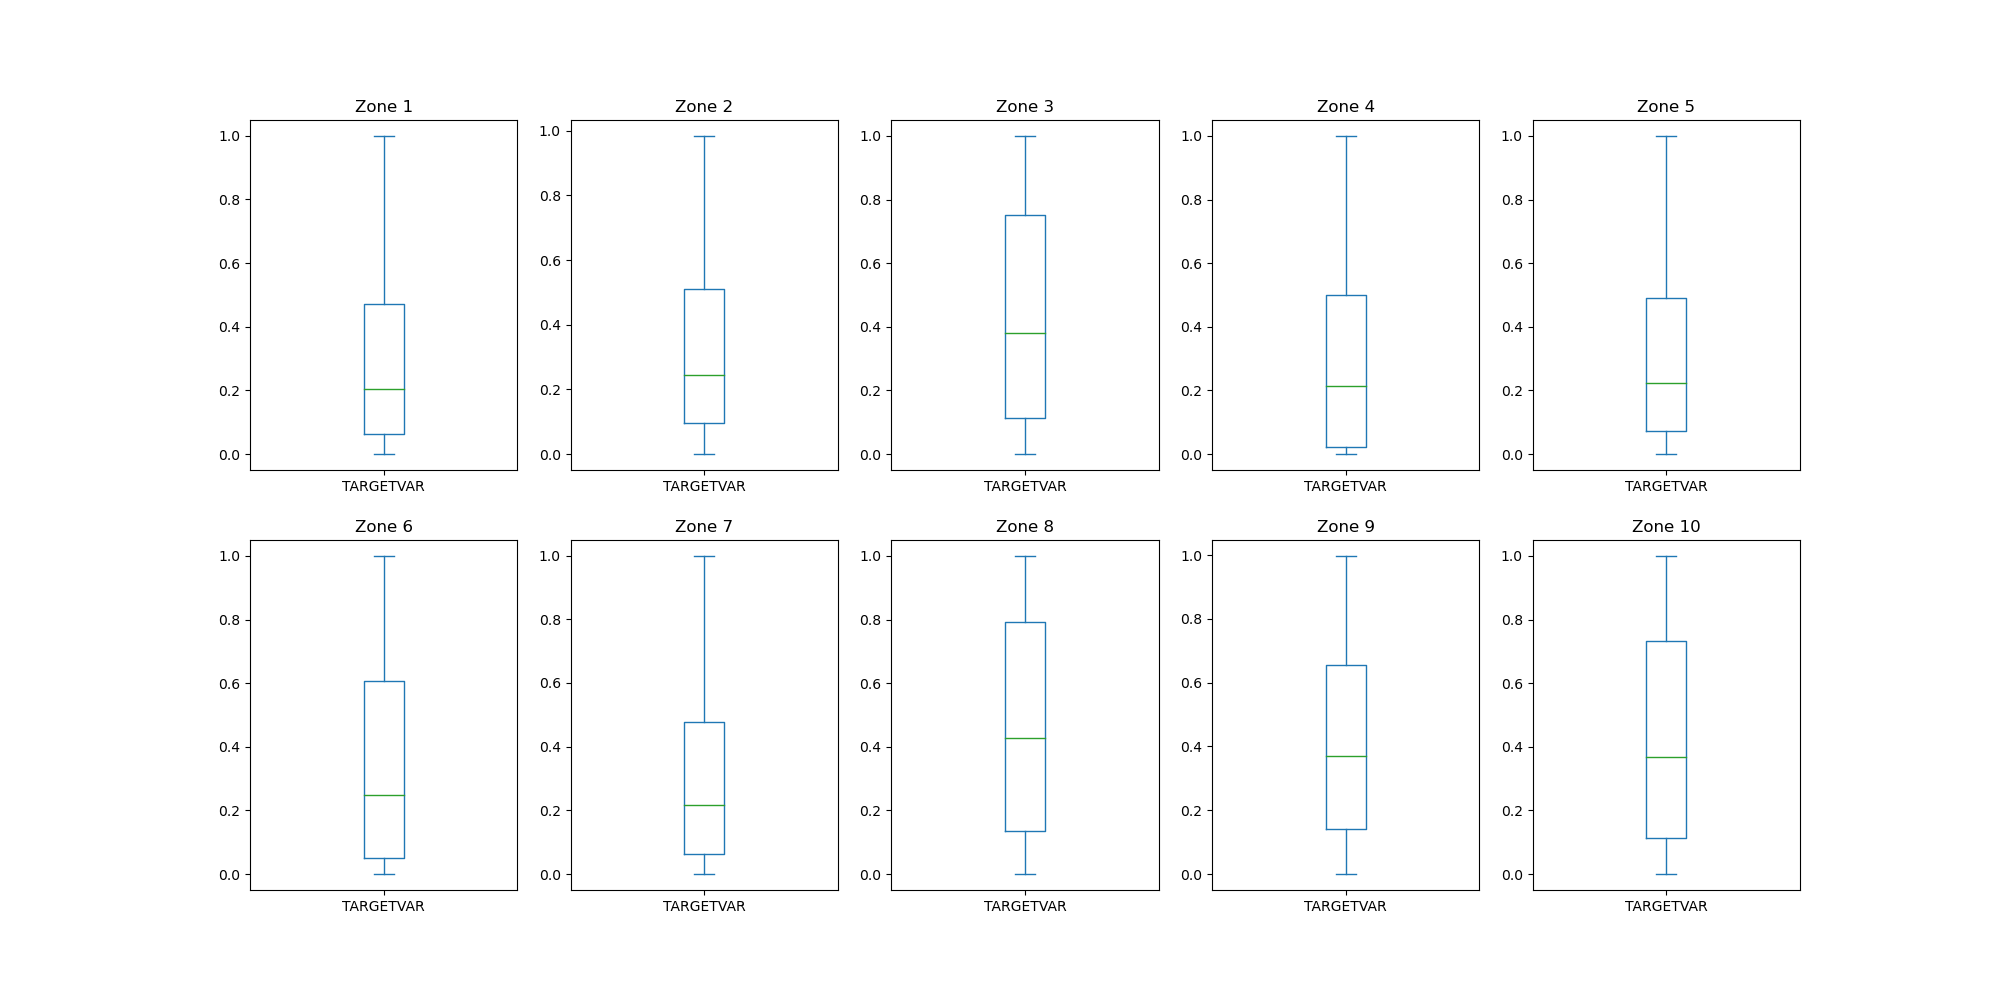
\includegraphics[width=.6\textwidth]{figs/boxplots_Y.png}
    \caption{Boxplot of TARGETVAR values in Y\_i zones}
    \label{fig:boxplot_Y}
\end{figure}

On one hand, as the data in the \verb|Y_i.csv| zones was normalized, it is as expected that we didn't find outliers in it. On the other hand, by diving into the boxplots for the variables in the \verb|X_i.csv| files, we clearly detect some outliers (using the \verb|boxplot.py| file with the basic data) : 

\begin{figure}[H]
    \centering
    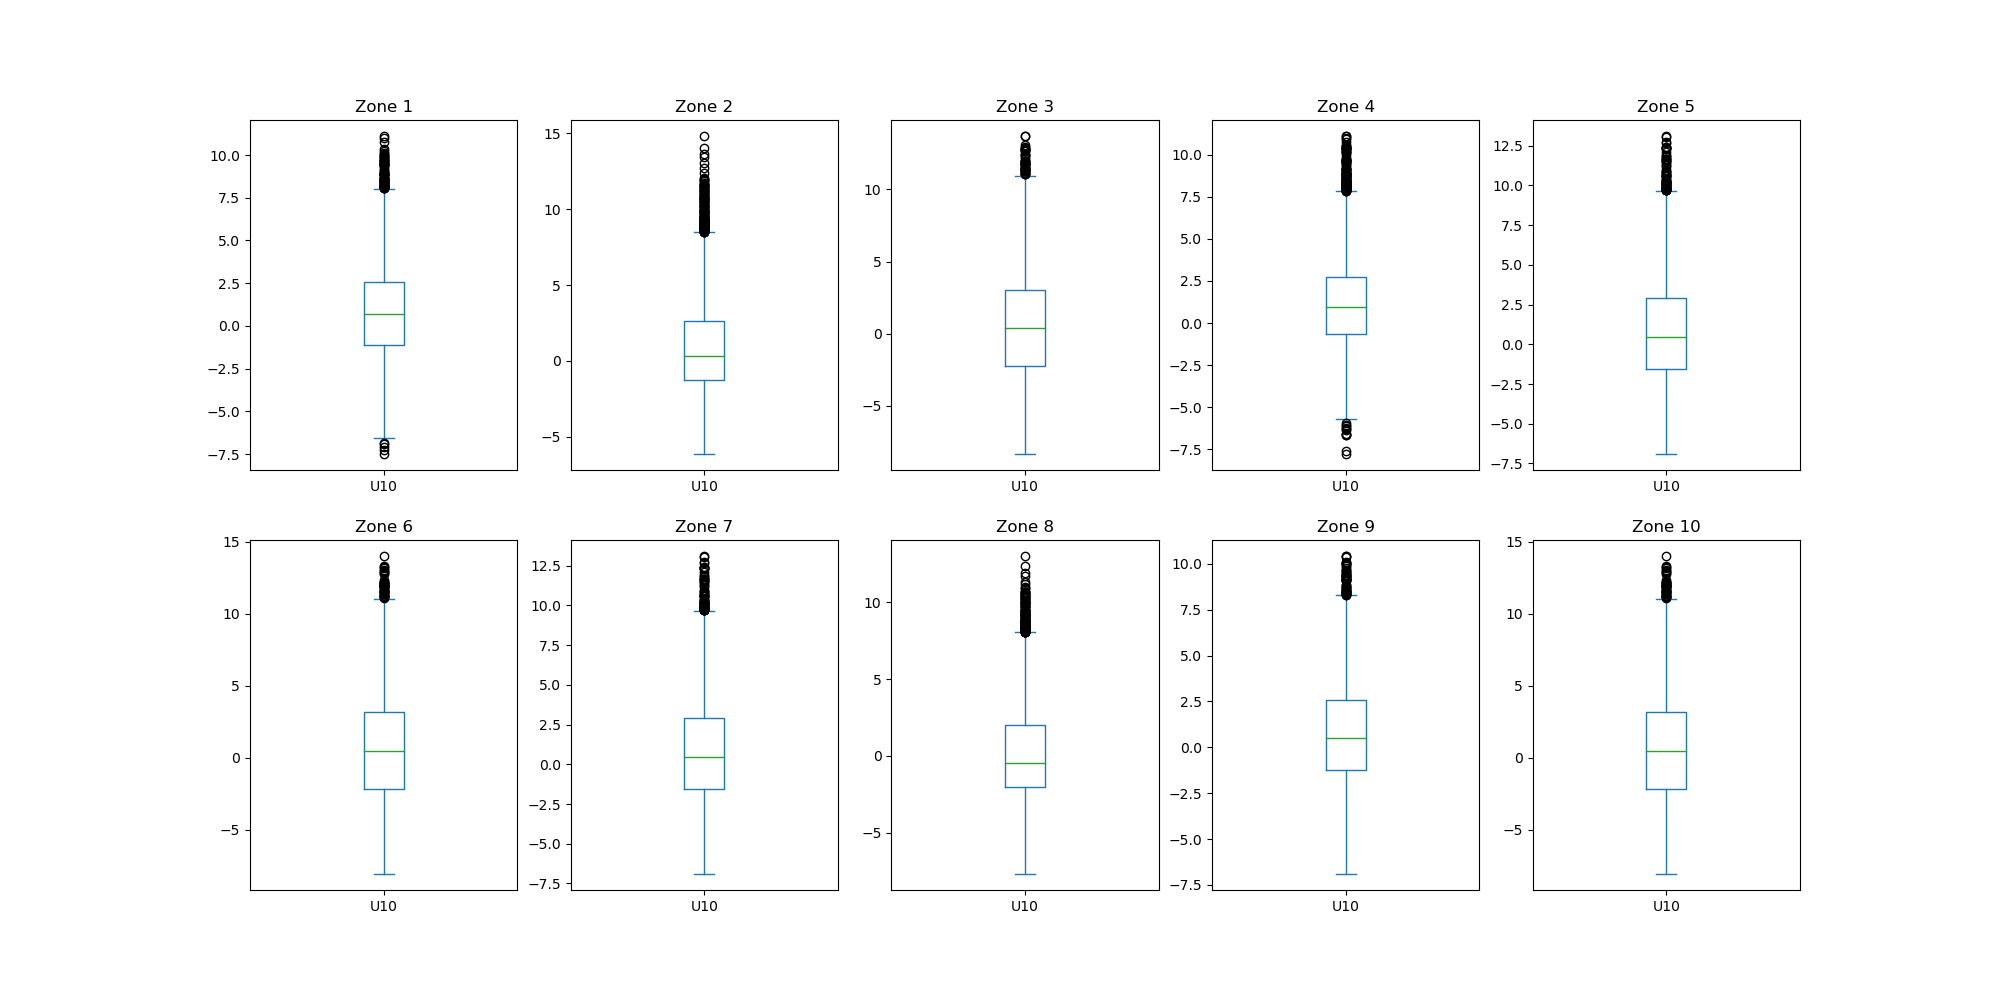
\includegraphics[width=.7\textwidth]{figs/boxplots_X_u10.png}
    \caption{Boxplot of U10 values in X\_i zones}
    \label{fig:boxplot_X_u10}
\end{figure}

\begin{figure}[H]
    \centering
    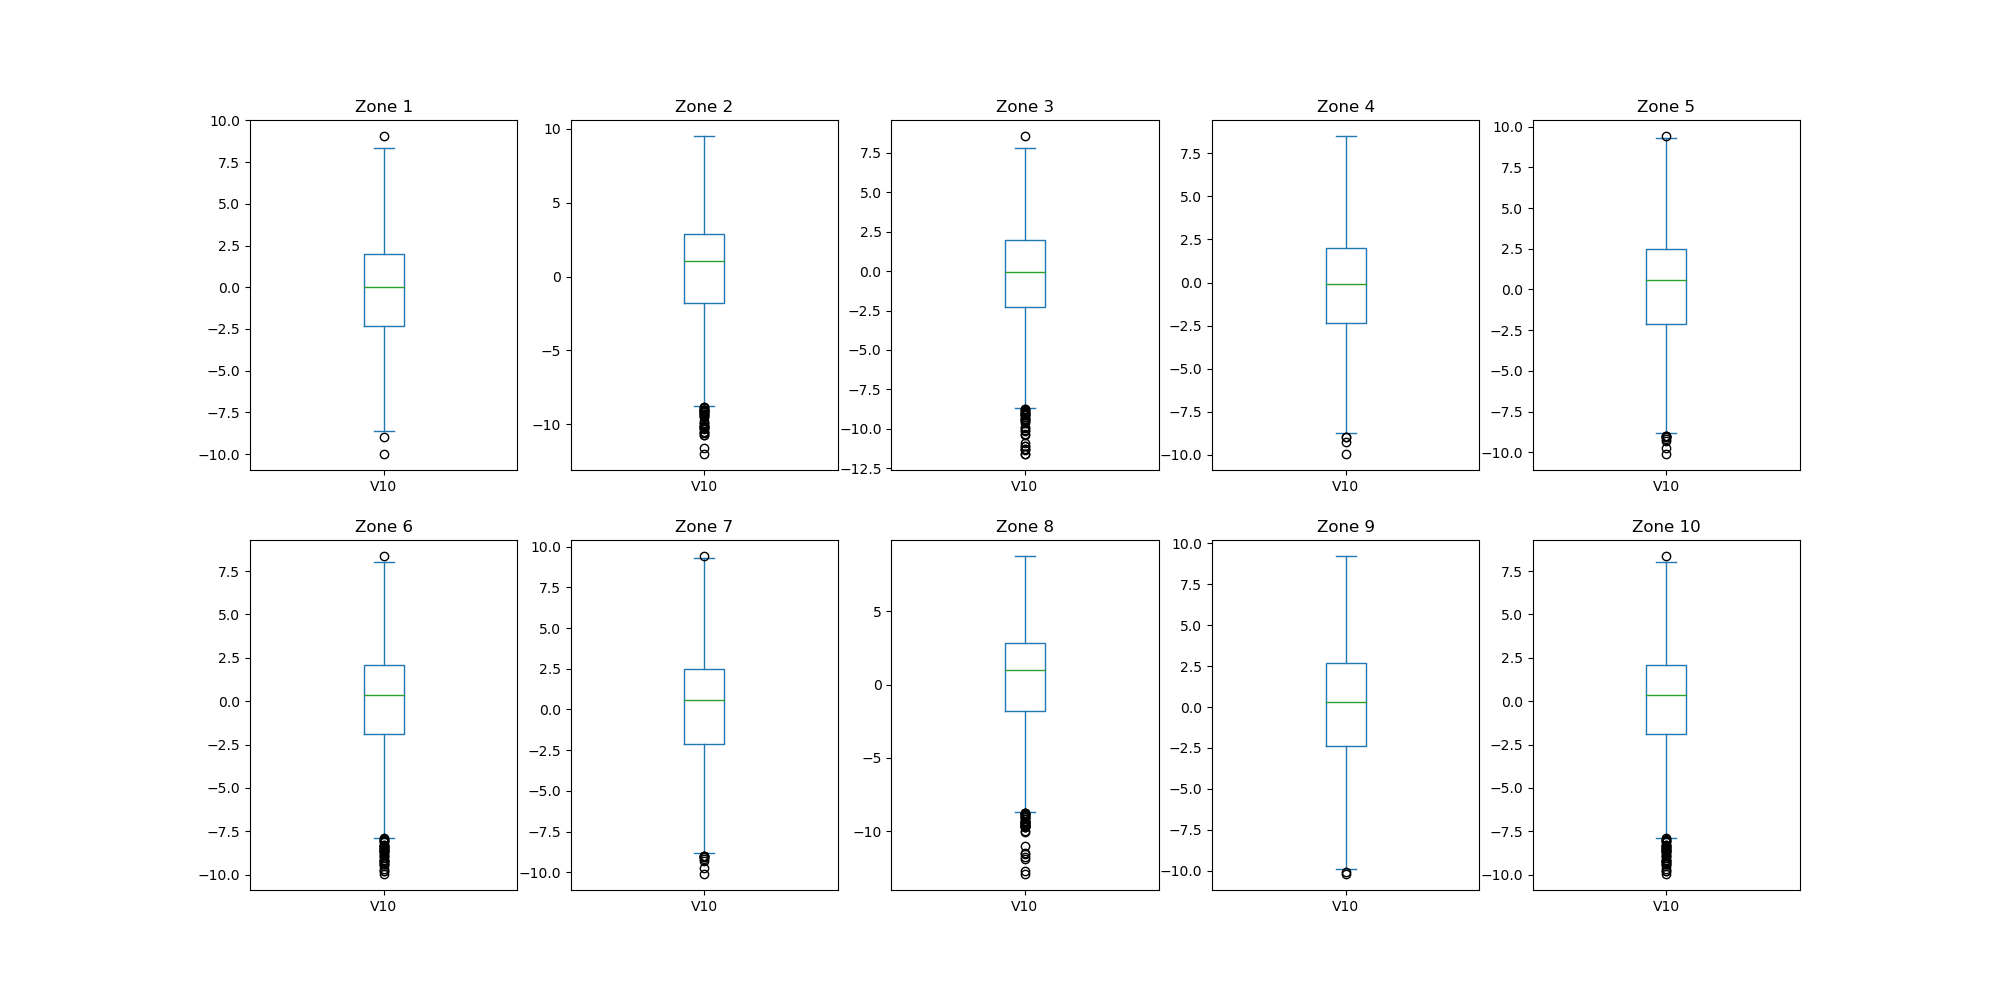
\includegraphics[width=.7\textwidth]{figs/boxplots_X_v10.png}
    \caption{Boxplot of V10 values in X\_i zones}
    \label{fig:boxplot_X_v10}
\end{figure}

\begin{figure}[H]
    \centering
    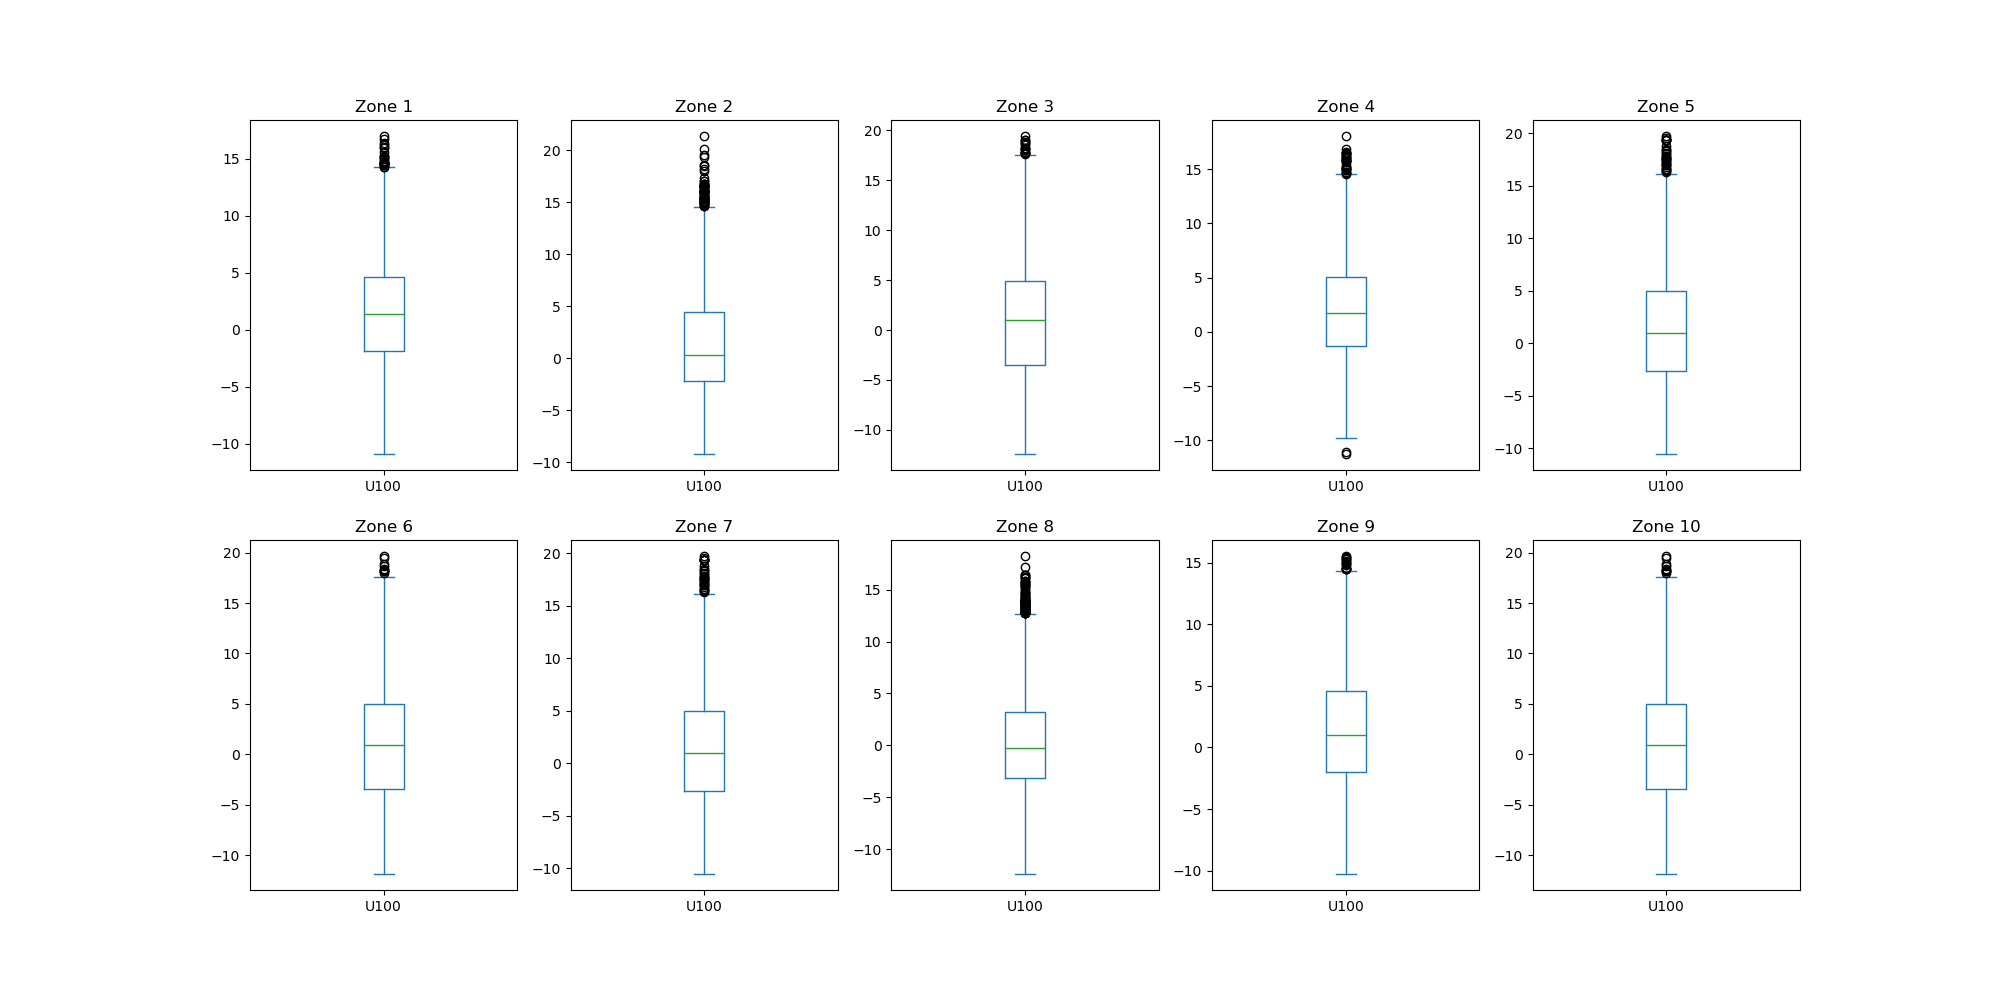
\includegraphics[width=.7\textwidth]{figs/boxplots_X_u100.png}
    \caption{Boxplot of U100 values in X\_i zones}
    \label{fig:boxplot_X_u100}
\end{figure}

\begin{figure}[H]
    \centering
    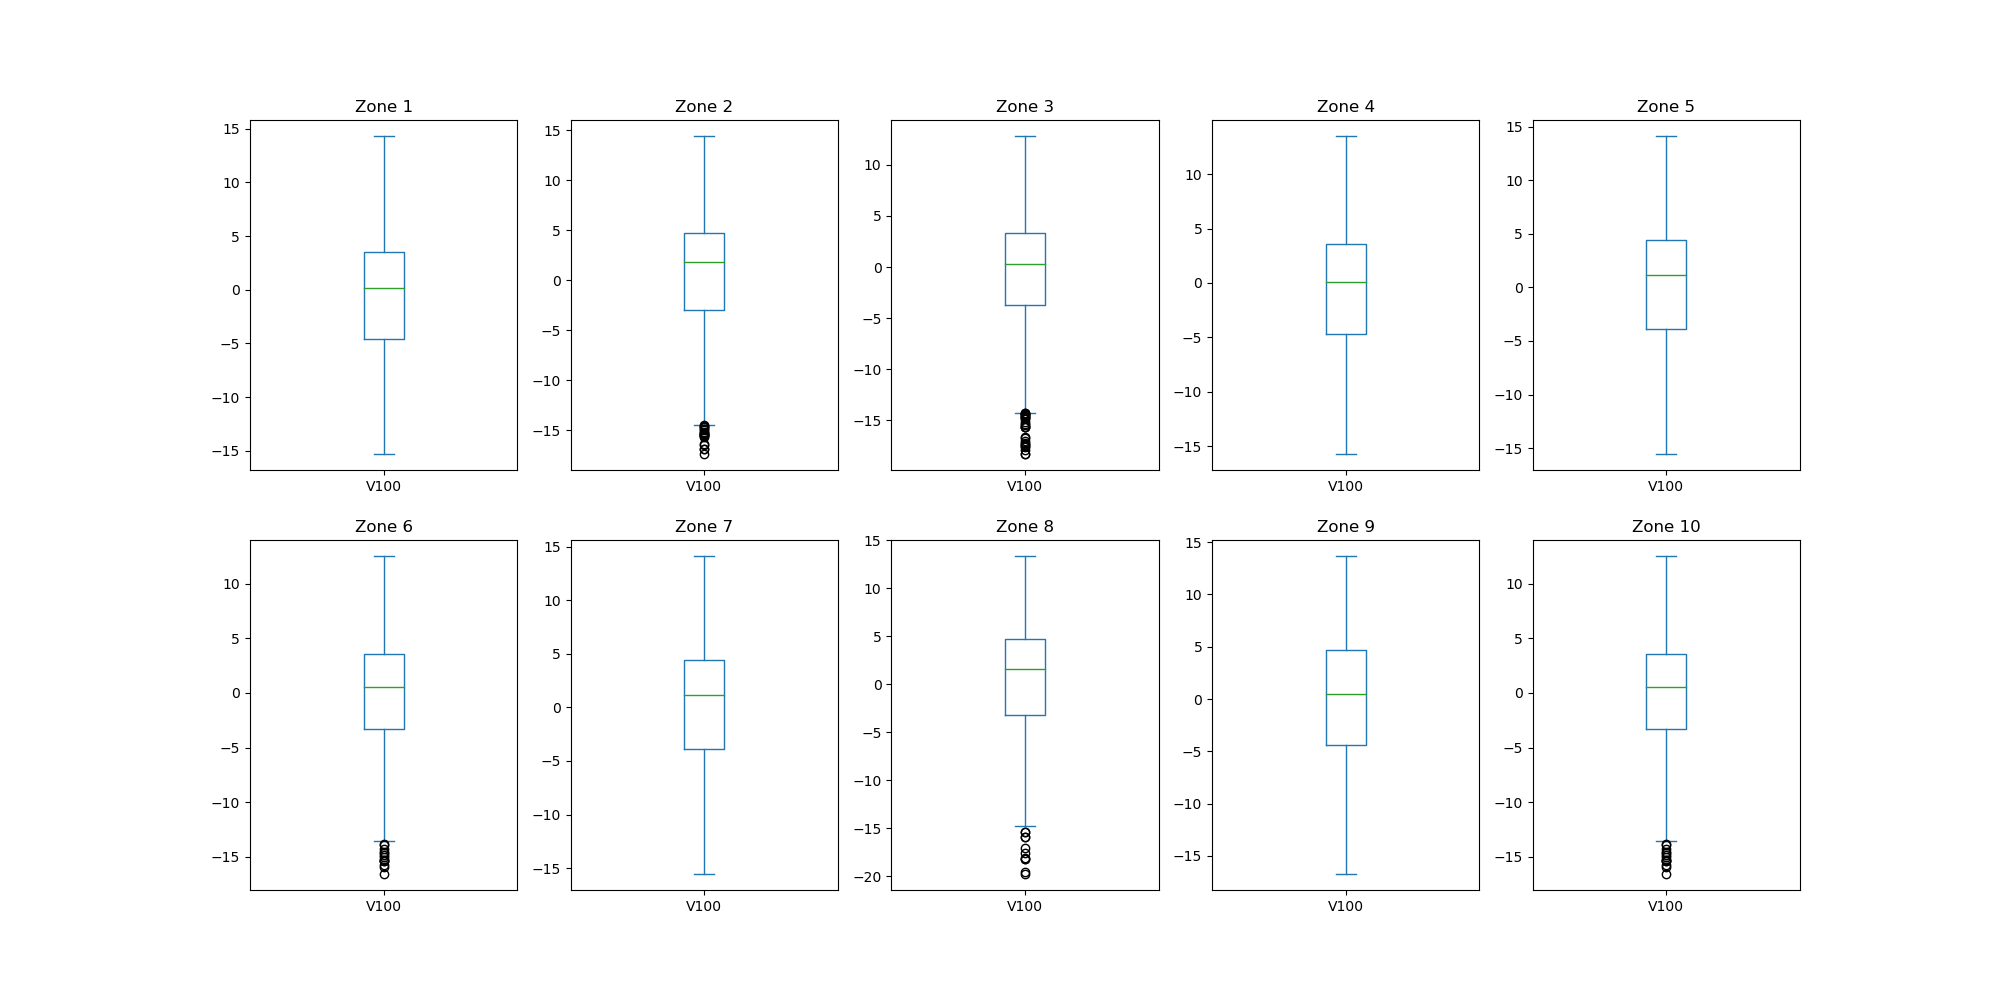
\includegraphics[width=.7\textwidth]{figs/boxplots_X_v100.png}
    \caption{Boxplot of V100 values in X\_i zones}
    \label{fig:boxplot_X_v100}
\end{figure}

We then needed to handle these outliers before fitting our models. This is done in the \verb|data.py| file using the \verb|handle_outliers| function by fixing the value of each outlier to the nearest non-outlier value in the dataframe. Indeed, in regression algorithm, handling the data is the first big step as outliers may induce the algorithm to perform a lot more differently. Here's the resulting boxplot for the \verb|U10| variable :

\begin{figure}[H]
    \centering
    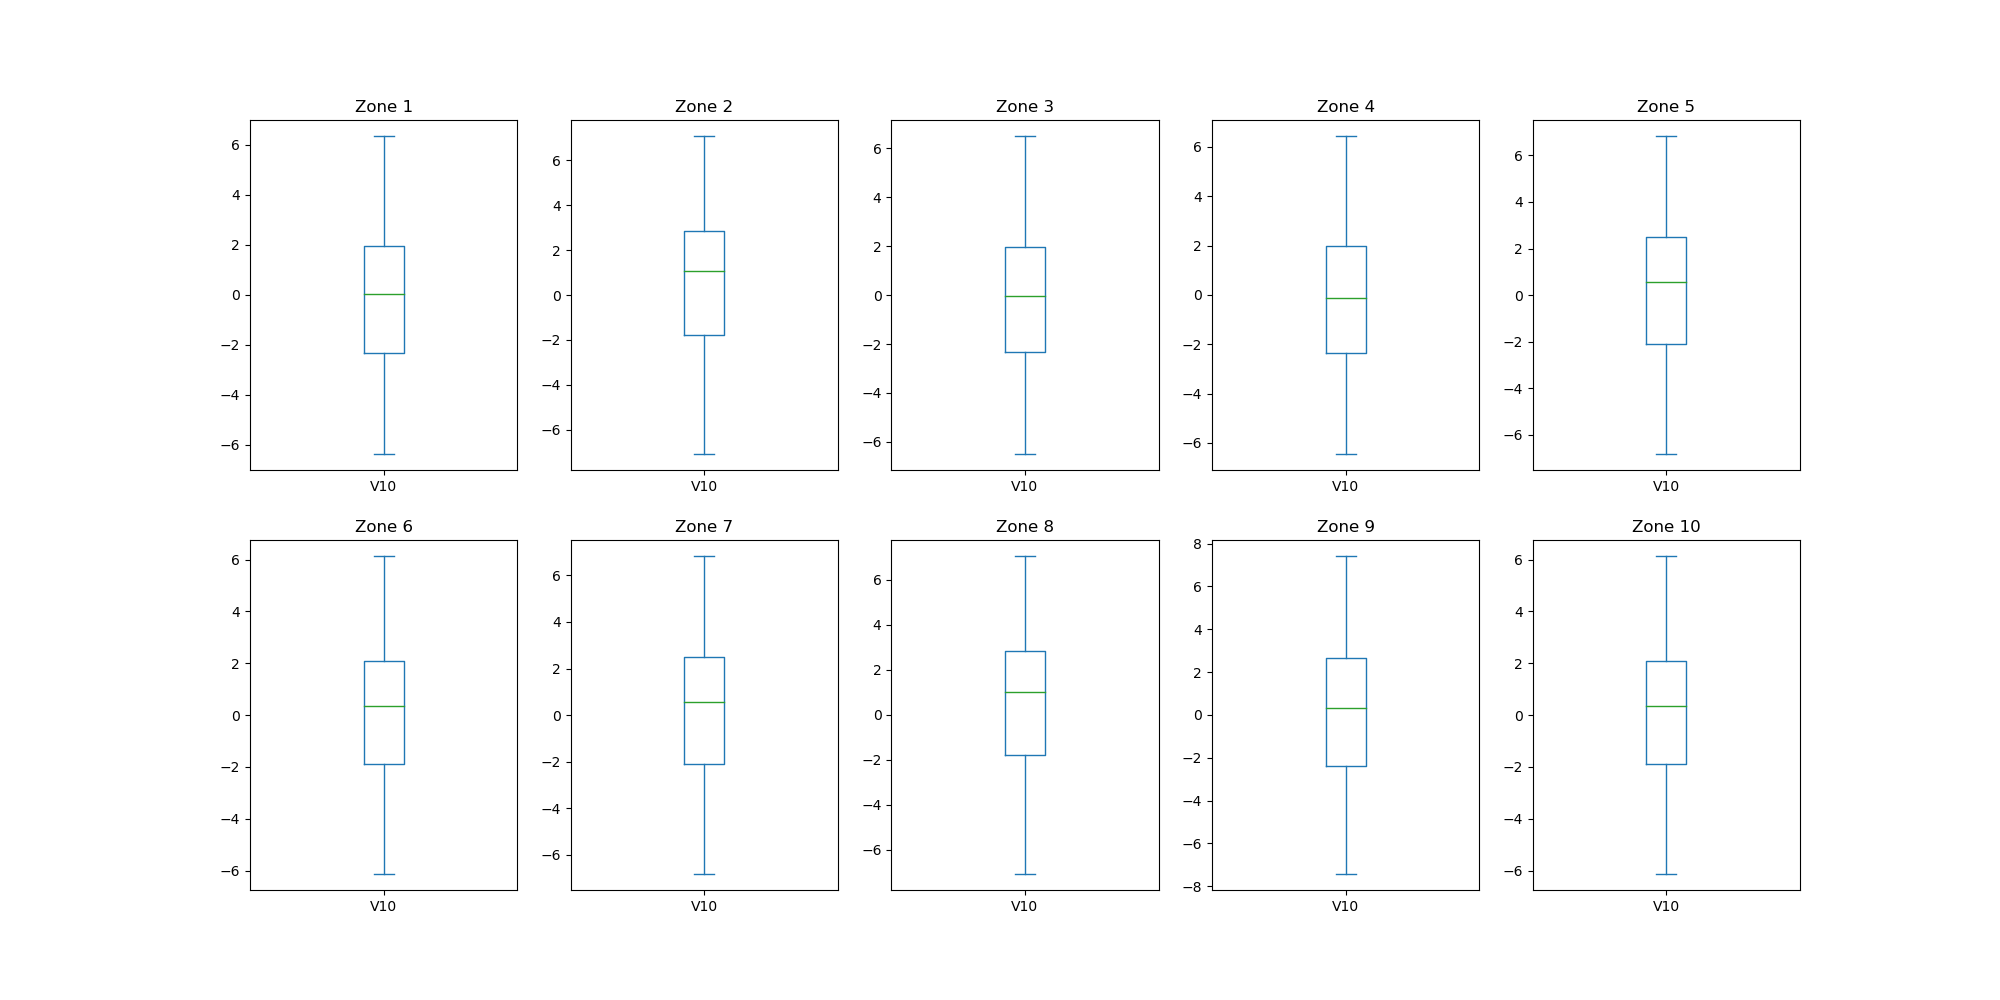
\includegraphics[width=.7\textwidth]{figs/boxplots_X_v10_handled.png}
    \caption{Boxplot of U10 values in X\_i zones after outlier handling}
    \label{fig:v10_handled}
\end{figure}